\documentclass[11pt]{article}
\usepackage[utf8]{inputenc}

\usepackage{geometry}
\geometry{a4paper}

\usepackage{graphicx}
\usepackage{hyperref}
\usepackage[parfill]{parskip}
\usepackage{amsmath, amssymb}
\usepackage{fdsymbol}
\usepackage{color,soul}

% remove section numbering
\makeatletter
\renewcommand{\@seccntformat}[1]{}
\makeatother

% make subsubsection italic
\usepackage{sectsty}
\subsubsectionfont{\itshape}

\renewcommand{\arraystretch}{1.4}

\title{Probability Theory \& Statistics}
\date{}
\author{}

\begin{document}
\maketitle
\clearpage

\section{Sample Spaces \& Events}

\subsection{Sample Spaces}

\emph{Sample spaces} are the set of all possible outcomes of an experiment. 
The following are a few examples of sample spaces

\begin{itemize}
\item 
the set of all 52 cards in a card deck: 
\(S_{1} = \{A\varheartsuit, A\vardiamondsuit,\ldots\}\)
\item 
the set of tomorrow's weather conditions: 
\(S_{2} = \{ Sunny,\ Overcast,\ldots\}\)
\item 
the set of all combinations of 2-flip coin experiments: 
\(S_{3} = \{HH, HT, TT, TH\}\)
\item 
the set of all possible temperatures (in Kelvin) in Bedford: 
\(S_{4} = \{T \in \mathbb{R}, \, T \geq 0\}\)
\end{itemize}

The last example uses \emph{set builder notation} which is mathematical shorthand notation 
for saying ``all of the positive decimal temperatures''.%
\footnote{Decimals with an infinite precision.}

\subsection{Events}

\emph{Events} are subsets of sample spaces.
A possible subset from \(S_{3}\) is the event ``at least one head is observed'', 
that is, \(A_{H} = \left\{HH, HT, TH\right\} \subset S_{3}\). 
We say that \emph{\(A_{H}\) occurred} if the actual outcome 
of an experiment is in \(A_{H}\). 
If we perform an experiment and flip a coin twice, 
observing that the first outcome is a head, 
and the second outcome is a tail, 
the event ``at least one head is observed'' has occurred.

\begin{figure}[h!]
\centering
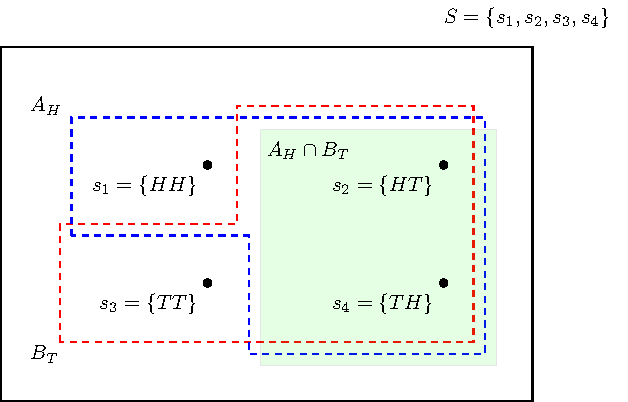
\includegraphics[width=0.6\linewidth]{tikz/figure1}
\caption{Sample space \(S\) of 2-flip coin outcomes \(s_{j}\), 
and the events \(A_{H}\): ``at least one head is observed'' in blue, 
\(B_{T}\): ``at least one tail is observed'' in red,
and their union \(A_{H} \cap B_{T}\) ``at least one head \emph{and} one tail is observed'' in green.}
\label{fig:coinflip}
\end{figure}

\subsection{Finite Sample Spaces}

\emph{Finite sample spaces} and their \emph{outcomes,} \(s_{j}\), 
can be visualized as marbles, 
with events, 
collections of marbles. 
It's useful to think of a sample space 
as a bag that contains marbles that each represent 
an outcome in an experiment. 
Performing the experiment corresponds to reaching 
into the bag and choosing a marble, 
where the chance of choosing any given marble 
is the same or \emph{equally likely}.%
\footnote{%
The source of the randomness is \emph{random sampling}.} 
We will see later that this can be generalized to smaller 
or larger marbles where their \emph{mass} makes them more or
less likely to be chosen.

Figure \ref{fig:coinflip} is the sample space of a 2-flip coin experiment.
The enclosing boxes are events, 
collections of outcomes that are subsets of the sample 
space corresponding to ``at least 1 head is observed'' or 
``at least 1 tail is observed'' observed in the 2-flip sequence. 
The shaded box is the event that at least 1 head \emph{and} 1 tail is observed,
\begin{align}
A_{H} \cap B_{T} = \{HT, TH\}.
\end{align}
The symbol \(\cap\) is used to denote the \emph{intersection} of (the outcomes of) events,
the outcomes shared by two events.

\subsection{Naïve Probability}

\subsubsection{Definition}

The \emph{naïve probability} that an event \(A\) 
occurs (on a finite sample space) is 
the number of outcomes favourable to \(A\) divided by the total number of outcomes. 
Using the same 2-flip coin example, 
the naïve probability of event \(A_{H}\), 
that ``at least 1 head is observed,''
can be calculated as
\begin{align}
P\left( A_{H} \right) = \frac{\left| A_{H} \right|}{\left| S_{3} \right|} = 
\frac{\left| \left\{ HH, HT,TH \right\} \right|}{|\left\{ HH,HT,TT,TH \right\}|} = 3/4.
\end{align}
The \emph{bar notation} \(|\cdot|\), 
denotes the \emph{size of a set}, 
for example \(A = \{HH, TT\}\) 
has \(|A| = 2\).
Relating the naïve probability to the bag of marbles interpretation,
assigns a mass \(1/|S|\) to each of the marbles, 
and a total mass \(P(S) = 1\).

\subsubsection{Limitations}

Naïve probability is often a good model to start with, for example:

\begin{itemize}
\item
When there is symmetry, e.g., physical symmetry like in a coin, 
or choosing a card at random from a deck 
(no single card prefers to be picked over any other card)
\item
By design -- it's a model assumption
\end{itemize}

But it has limitations

\begin{itemize}
\item
There is no difference between the probability of ``there is life on Mars'' 
and ``there is intelligent life on Mars''. 
(We would expect that the second statement is far less likely, 
but it is still ½ by the naïve definition of probability)
\item
Sample spaces with an infinite number of possible 
outcomes (possible temperature in Bedford tomorrow) have 0 probability of any single
outcome occurring since \(\left| S_{4} \right| = \infty\)
\end{itemize}

\subsection{Conditioning}

Events that share possible outcomes (they \emph{intersect}) change the probabilities
associated with them if either of the events occur 
(we will later formally define this as ``dependence'', 
but it's more useful to think of the events as containing information about each other).

\begin{figure}[h!]
\centering

\includegraphics[width=0.6\linewidth]{tikz/figure2}
\caption{%
A 2-flip coin experiment outcome space after observing \(B_{T}\): ``at least 1 tail is observed'',
means its complement the event \(\overline{B_{T}}\): ``no tails are observed'' cannot occur.}
\label{fig:conditioning}
\end{figure}

For a 2-flip coin experiment, 
if the event ``at least 1 tail is observed'' occurs, 
it's impossible for the outcome \(s_{1} = \{HH\}\) to occur. 
The probability of the event ``at least 1 head is observed'' is then changed (it is less likely).

We define the \emph{conditional probability}, 
i.e., the probability of an event \(A\) occurring given an event \(B\) has occurred, as
\begin{align}
P\left( A \middle| B \right) := \frac{P(A \cap B)}{P(B)}
\end{align}
To see why this is true, 
consider the 2-flip coin experiment again. 
Upon obtaining the information that ``at least 1 tail'' has been observed in an actual experiment 
-- conditioning on \(B_{T}\), 
we can remove the marbles from the sample space \(S_{3}\) that aren't in \(B_{T}\) 
since they are incompatible with the knowledge that \(B_{T}\) has occurred.

Elements ``not in'' any given set are denoted with the \emph{complement notation} \(\overline{A}\). 
In the 2-flip coin experiment, 
the complement of ``at least 1 tail'' is ``no tails'',
\begin{align}
\overline{B_{T}} = \{ HH\}
\end{align}

Having removed this event from the sample space, 
the total mass of the marbles that remain in the event \(A_{H}\), 
``at least 1 head'', 
is \(P\left( A_{H} \cap B_{T} \right) = 2/4 = 1/2\). 
But only 3 outcomes are left in the sample space totalling a mass 3/4, 
and each outcome must be equally likely, i.e., 
for a probability to be valid, 
the total mass of marbles must sum to 1. 
To achieve this, 
we \emph{renormalize} the sample space by dividing through by 
the probability of the event \(B_{T}\)
\begin{align}
P\left( A_{H} \middle| B_{T} \right) = 
\frac{P\left( A_{H} \cap B_{T} \right)}{P(B_{T})} = 
\frac{2/4}{3/4} = 2/3.
\end{align}
This assigns the correct ``mass'' to the event \(A_{H}\) 
conditional on the occurrence of the event \(B_{T}\).

\section{Discussion}

\subsection{Random Variables}

\emph{How are events related to random variables and distributions?}

Random variables are functions, \(X(\cdot)\), 
that map elements in
the outcome space to the real number line, i.e., \(X(s_j) = x\), for \(x \in \mathbb{R}\).
Distributions provide the ``blueprint'' for the probability of events like \(\{X=x\}\).

\section{Practice}

\subsection{Finite Sample Spaces}

1a) 2 coins were flipped and at least one of them landed heads. 
What is the probability that both coins landed heads?

1b) Imagine \(m\) coins flipped at the same time and their outcomes recorded. 
What is the probability that all the coins land heads, 
given at least one of them landed heads?

2a) Show that the probability of the complement of an event \(A\) 
can be calculated from the naïve probability as
\begin{align}
P\left( \overline{A} \right) = 1 - P(A).
\end{align}

2b) Consider the sample space of 52 playing cards, \(S_{1}\). 
How many possible events (subsets of \(S_{3}\)) are there?

\subsection{Conditioning}

3a) Using the definition of conditional probability, derive \emph{Bayes' Theorem} 
that relates the probability of event \(A\) given \(B\) 
has occurred with the probability of \(B\) given \(A\) has occurred
\begin{align}
P\left( A \middle| B \right) = \frac{P\left( B \middle| A \right)P(A)}{P(B)}
\end{align}

3b) Show that \(P\left( A \middle| A \right) = 1\).

\end{document}
